\section{Auswertung}
\label{sec:Auswertung}
\subsection{Untersuchung des Acrylblocks mit einer Schieblehre}
Die gemessene Höhe des Acrylblocks beträgt:
\begin{eqution*}
  h =  80.25\si{\milli\meter}
\end{eqution*}
Die Bohrungen des Acrylblocks werden mit einer Schieblehre vermessen.
Die erhaltenen Werte sind in Tabelle \ref{tab:schieb} eingetragen.
\begin{table}[H]
    \caption{Messung der Borungen mit einer Schieblehre.}
    \label{tab:schieb}
    \centering
    \begin{tabular}{S[table-format=2] S[table-format=2.2(0)e0] S[table-format=2.2(0)e0] S[table-format=2.2(0)e0]  }
        \toprule
        {Bohrung} & {Oberkante$/\si{\milli\meter}$} & {Unterkante$/\si{\milli\meter}$} &{Durchmesser$/\si{\milli\meter}$} \\
        \midrule
             1 & 19.20  & 59.65 & 1.40\\
             2 & 17.45  & 61.35 & 1.45\\
             3 & 61.05  & 13.45 & 5.75\\
             4 & 53.70  & 21.70 & 4.85\\
             5 & 46.30 & 30.95 & 3.00\\
             6 & 38.70 & 38.65 & 2.90\\
             7 & 30.75 & 46.65 & 2.85\\
             8 & 22.80 & 54.65 & 2.80\\
             9 & 14.80 & 62.70 & 2.75\\
             10 & 6.85 & 70.65 & 2.75\\
             11 & 56.40 &  15.20 & 8.65\\
        \bottomrule
    \end{tabular}
\end{table}
\noindent
\subsection{Untersuchung des Acrylblocks mit A-Scan}
Der Acrylblock wird wie in der Durchführung beschrieben mit dem A-Scan vermessen.
Die Schallgeschwindigkeit in Acryl beträgt $c=2730$\cite{acryl}.
Die Eindringunstiefe kann, dann nach Gleichung\eqref{eq:schall} brechnet werden.
Die erhaltenen Werte sind in Tabelle\ref{tab:a-scan} eingetragen.
Dabei muss die Abweichung, welche durch die Schutzschicht der Sonde entsteht, beachtet werden.
Diese beträgt:
\begin{equation*}
  \delta h = 0.25\si{\milli\meter}
\end{equation*}
\begin{table}[H]
    \caption{Messung der Bohrungen mit dem A-Scan .}
    \label{tab:a-scan}
    \centering
    \begin{tabular}{S[table-format=2] S[table-format=2.2(0)e0] S[table-format=2.2(0)e0] S[table-format=2.2(0)e0] }
        \toprule
        {Bohrung} & {Oberkante$/\si{\milli\meter}$} & {Unterkante$/\si{\milli\meter}$&{Durchmesser$/\si{\milli\meter}$} \\
        \midrule
             1 & 19.82  & 60.58 & -0.15\\
             2 & 17.70  & 61.13 & 1.42\\
             3 & 59.95  & 13.22 & 7.08\\
             4 & 53.68  & 21.61 & 4.96\\
             5 & 46.27 & 29.99 & 3.99 \\
             6 & 38.75 & 38.65 & 2.85\\
             7 & 30.64 & 46.67  & 2.94\\
             8 & 22.77 & 54.52 & 2.96 \\
             9 & 14.77 & 62.73 &  2.75 \\
             10 & 7.01 & / & /\\
             11 & 55.43 &  15.08  & 9.74\\
        \bottomrule
    \end{tabular}
\end{table}
\noindent
Erhält ein Element der Tabelle ein "/", so konnte kein Wert an der entsprechenden Stelle gemessen werden.
Die Bohrungen $1$ und $2$ werden erneut vermessen. Die dafür verwendete Sonde besitzt ein Auflösungsvermögen von $\SI{4}{\mega\hertz}$.
Die Werte sind in Tabelle \ref{tab:aufl} eingetragen.
\begin{table}[H]
    \caption{Messung des Auflösungsvermögen.}
    \label{tab:aufl}
    \centering
    \begin{tabular}{S[table-format=2] S[table-format=2.2(0)e0] S[table-format=2.2(0)e0]  }
        \toprule
        {Bohrung} & {Oberkante$/\si{\milli\meter}$} & {Unterkante$/\si{\milli\meter}$} \\
        \midrule
             1 & 19.82  & /\\
             2 & 17.70  & /\\
        \bottomrule
    \end{tabular}
\end{table}
\noindent
\subsection{Untersuchung des Acrylblocks mit B-Scan}
Die Messung wird nach der Durchführung beschrieben ausgeführt.
\begin{figure}[H]
  \centering
  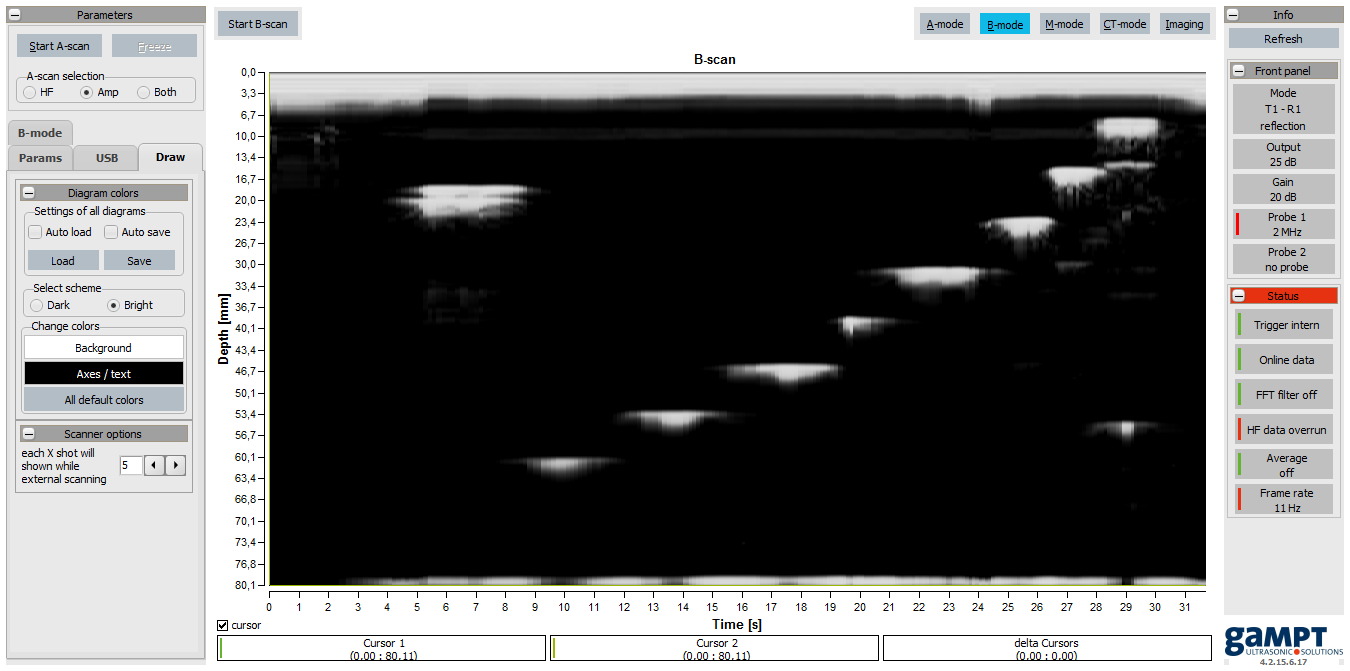
\includegraphics[width=0.8\textwidth]{content/bscan-2mhz_oberseite.png}
  \caption{Messung des Acrylblock von der Oberkante.}
  \label{fig:obs}
\end{figure}
\begin{figure}[H]
  \centering
  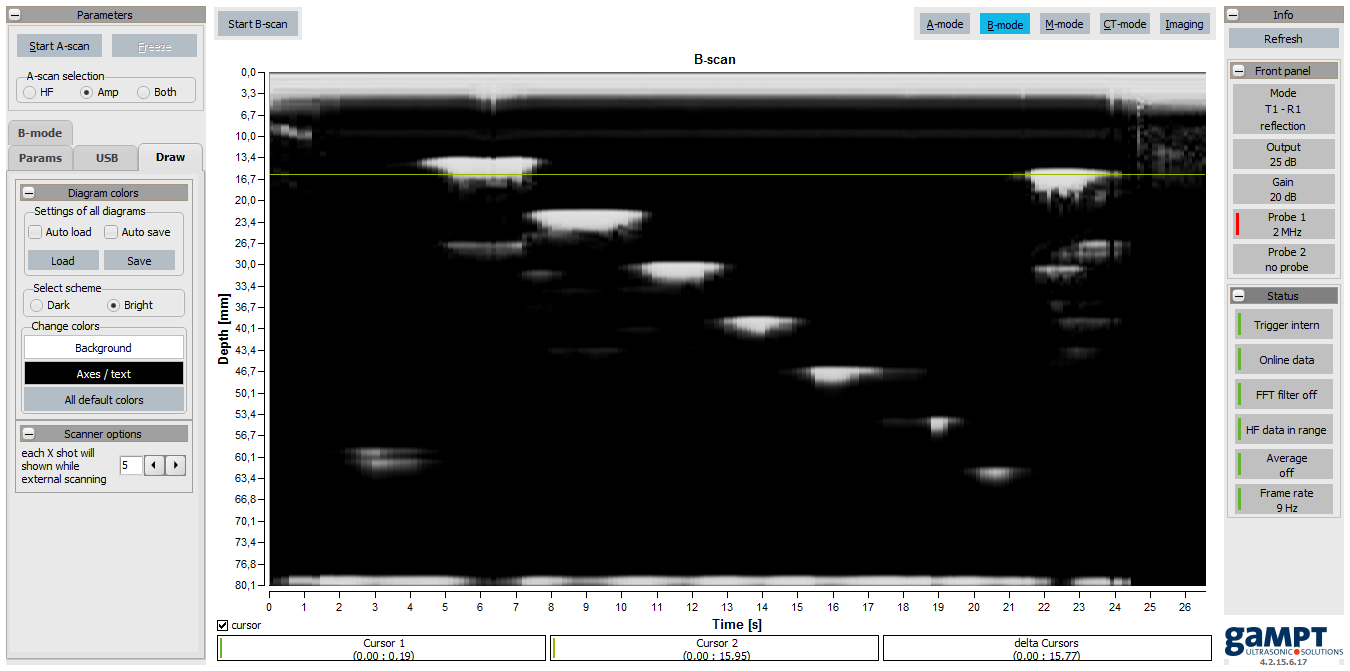
\includegraphics[width=0.8\textwidth]{content/bscan-2mhz_unterseite.png}
  \caption{Messung des Acrylblock von der Unterkante.}
  \label{fig:unts}
\end{figure}
Aus der Aufnahme \ref{fig:obs} und der Aufnahme \ref{fig:unts} können die Bohrungen lokalisiert werden.
Die erhaltenen Werte sind in Tabelle \ref{tab:b-scan} eingetragen.
\begin{table}[H]
    \caption{Messung der Bohrungen mit dem B-Scan .}
    \label{tab:b-scan}
    \centering
    \begin{tabular}{S[table-format=2] S[table-format=2.2(0)e0] S[table-format=2.2(0)e0] S[table-format=2.2(0)e0]  }
        \toprule
        {Bohrung} & {Oberkante$/\si{\milli\meter}$} & {Unterkante$/\si{\milli\meter}$}&{Durchmesser$/\si{\milli\meter}$} \\
        \midrule
             1 & 20.18  & 59.92 & 0.15\\
             2 & 18.58  & 61.85 & -0.18\\
             3 & 61.68  & 13.64 &  4.93\\
             4 & 54.02  & 22.57 & 3.66\\
             5 & 46.68 & 30.71  & 2.86 \\
             6 & 39.16 & 39.34  & 1.75\\
             7 & 31.35 & 47.15  & 1.75\\
             8 & 23.37 & 55.13  & 1.75\\
             9 & 15.71 & 62.27  & 2.27\\
             10 & 8.05 & / & /\\
             11 & 56.01 &  15.87 &  8.37\\
        \bottomrule
    \end{tabular}
\end{table}
\noindent
\subsection{Untersuchung des kruden Herzmodells}
Das Herz hat einen Radius von $r_\text{Herz}=\SI{22.75}{\milli\meter}$.
Als Schallgeschwindigkeit für Wasser wurde ein Wert von $c=\SI{1484}{\meter\per\second}$ verwendet.
Die Werte für das Grundniveau und die Maximalausschlag sind in Tabelle \ref{maxschlag} aufgetragen.

\begin{table}[H]
    \caption{Messung des maximalen Ausschlags.}
    \label{maxschlag}
    \centering
    \begin{tabular}{S[table-format=2.2] S[table-format=2.2]}
        \toprule
        {Grundniveau$/\si{\milli\meter}$} &
        {Maximaler Ausschlag$/\si{\milli\meter}$} \\
        \midrule
        38.27             & 6.38 \\
        \bottomrule
    \end{tabular}
\end{table}
\noindent

Anschließend wird der simulierte Herzschlag untersucht und die Messerbegnisse in Tabelle \ref{tab:schlag} aufgetragen.
\begin{table}[H]
    \caption{Messung des Herzschlags.}
    \label{tab:schlag}
    \centering
    \begin{tabular}{S[table-format=2.2]}
        \toprule
        {Peaks ohne Grundniveau$/\si{\milli\meter}$} \\
        \midrule
            14.87 \\
            13.96 \\
            15.98 \\
            14.26 \\
            13.46 \\
            14.57 \\
            14.17 \\
            15.18 \\
            14.07 \\
            14.37 \\
            14.97 \\
            14.68 \\
            13.56 \\
            14.57 \\
            13.46 \\
            14.47 \\
            14.87 \\
            14.87 \\
            16.49 \\
            12.85 \\
        \bottomrule
    \end{tabular}
\end{table}
\noindent

Der Herzschlag wurde über eine Zeit von $\SI{27.8}{\second}$ gemessen.
Es ergibt sich somit eine mittlere Schlagauslenkung von
\begin{equation}
   \overline{h}_\text{Herz} = \SI{14.48\pm0.19}{\milli\meter}
\end{equation}
und
\begin{equation}
   \overline{\nu}_\text{Herz} = \SI{0.72}{\hertz}.
\end{equation}
Das Volumen eines Kugelschnittes lässt sich wie folgt berechnen:
\begin{align}
    V &= \frac{\pi h^2}{3}\left( \frac{3({r'}^2+h^2)}{2h} - h \right) \\
    \symup{\Delta}V &= \frac{\pi h^2}{2}(3{r'}^2+5h^2-2)\symup{\Delta}h
\end{align}
Wobei $r'$ der Radius der Herzmodells und $h$ die Auslenkungshöhe ist.
Somit ergibt sich ein mittlerer Herzstrom von
\begin{equation}
   \overline{Q}_\text{Herz} = V(\overline{h}_\text{Herz})\overline{\nu}_\text{Herz} = \SI{9.62\pm0.09e-6}{\meter\cubed\per\second}.
\end{equation}
